% =========================================================================
%  Metodologia e Resultados — IC Conforto Térmico Veicular (CFD + Redes Neurais)
%  Compilar com: pdflatex metodologia_resultados.tex  (2 passagens)
% =========================================================================
\documentclass[12pt, a4paper]{article}

\usepackage[utf8]{inputenc}
\usepackage[T1]{fontenc}
\usepackage[brazil]{babel}
\usepackage{amsmath, amssymb}
\usepackage{booktabs}
\usepackage{multirow}
\usepackage{graphicx}
\usepackage{xcolor}
\usepackage{siunitx}
\usepackage{todonotes}
\usepackage{subcaption}
\usepackage{bm}
\usepackage{geometry}
\usepackage{hyperref}

\geometry{margin=2.5cm}
\graphicspath{{../}}   % caminhos relativos à raiz do projeto

\sisetup{
  output-decimal-marker = {,},
  group-separator       = {.},
}

\newcommand{\andamento}{\textit{--}}

\title{%
  Modelos Substitutos Baseados em Redes Neurais Profundas\\
  para Predição de Campos de Escoamento em Cabines Veiculares
}
\author{%
  \textit{[Nome do autor]}\\
  Universidade Federal de Santa Catarina --- Centro Tecnológico de Joinville\\
  Orientador: \textit{[Nome do orientador]}
}
\date{\today}

% =========================================================================
\begin{document}
\maketitle
\tableofcontents
\newpage

% =========================================================================
\section{Metodologia}
\label{sec:metodologia}

\subsection{Base de Dados CFD}
\label{sec:dados}

Os dados de treinamento foram gerados por meio de simulações de Dinâmica dos
Fluidos Computacional (CFD) em regime permanente de uma cabine veicular
reconstruída a partir da geometria de referência de \cite{mao2018}.
O solver ANSYS Fluent foi utilizado com o modelo de turbulência RANS
$k$--$\omega$ SST e o método das ordenadas discretas (DOM) para modelagem
da transferência de calor por radiação.

Para cobrir o espaço operacional do sistema HVAC, foram definidos três fatores
de projeto: velocidade de insuflamento (\textit{Vel}), temperatura de
insuflamento (\textit{Tinsu}) e vazão volumétrica (\textit{Qinsu}).
Um total de \textbf{45 casos de simulação} foi gerado por meio de um
Planejamento de Experimentos (DOE) com amostragem por Hipercubo Latino (LHS),
garantindo cobertura uniforme do espaço de parâmetros.

\subsection{Variáveis de Entrada e Saída}
\label{sec:variaveis}

Cada ponto da malha CFD é descrito por seis variáveis de entrada e nove
variáveis alvo, conforme a Tabela~\ref{tab:variaveis}.

\begin{table}[htb]
\centering
\caption{Variáveis de entrada e saída da rede neural.}
\label{tab:variaveis}
\begin{tabular}{@{}llll@{}}
\toprule
\textbf{Papel} & \textbf{Variável} & \textbf{Descrição} & \textbf{Unidade} \\
\midrule
\multirow{6}{*}{Entrada}
  & $x$ & Coordenada espacial X & \si{\metre} \\
  & $y$ & Coordenada espacial Y & \si{\metre} \\
  & $z$ & Coordenada espacial Z & \si{\metre} \\
  & \textit{Vel}   & Velocidade de insuflamento & \si{\metre\per\second} \\
  & \textit{Tinsu} & Temperatura de insuflamento & \si{\kelvin} \\
  & \textit{Qinsu} & Vazão volumétrica de entrada & \si{\metre\cubed\per\second} \\
\midrule
\multirow{9}{*}{Saída}
  & $p$      & Pressão manométrica         & \si{\pascal} \\
  & $u$      & Velocidade em X             & \si{\metre\per\second} \\
  & $v$      & Velocidade em Y             & \si{\metre\per\second} \\
  & $w$      & Velocidade em Z             & \si{\metre\per\second} \\
  & $T$      & Temperatura do ar           & \si{\kelvin} \\
  & $G$      & Radiação incidente          & \si{\watt\per\metre\squared} \\
  & $T_{r}$  & Temperatura radiante        & \si{\kelvin} \\
  & $q_{r}$  & Fluxo de calor radiativo    & \si{\watt\per\metre\squared} \\
  & $v_{r}$  & Velocidade resultante       & \si{\metre\per\second} \\
\bottomrule
\end{tabular}
\end{table}

\subsection{Divisão por Regiões da Cabine}
\label{sec:regioes}

O domínio volumétrico da cabine foi segmentado em oito regiões de análise,
alinhadas às zonas corporais relevantes para o cálculo de índices de conforto
térmico (PMV/PPD, Temperatura Radiante Média):

\begin{itemize}
  \item \textbf{fp\_head}: região da cabeça do passageiro dianteiro;
  \item \textbf{lrp\_head}: região da cabeça do passageiro traseiro esquerdo;
  \item \textbf{rrp\_head}: região da cabeça do passageiro traseiro direito;
  \item \textbf{mt\_head}: região da cabeça do motorista;
  \item \textbf{mt\_core}: região do tronco do motorista;
  \item \textbf{mt\_l\_foot}: região do pé esquerdo do motorista;
  \item \textbf{mt\_r\_foot}: região do pé direito do motorista;
  \item \textbf{outlet}: região de saída de ar.
\end{itemize}

Para cada região treina-se uma rede neural independente, pois os campos de
velocidade, temperatura e radiação diferem substancialmente entre zonas
(e.g., região dos pés versus cabeça do motorista).

\subsection{Arquitetura da Rede Neural}
\label{sec:arquitetura}

Adotou-se uma arquitetura de Perceptron Multicamadas (MLP) totalmente
conectado, implementada em TensorFlow/Keras. A estrutura é:

\begin{equation}
  \hat{\mathbf{y}} = f_L \circ \cdots \circ f_1(\text{Norm}(\mathbf{x}))
  \label{eq:mlp}
\end{equation}

\noindent onde \(\text{Norm}(\cdot)\) é uma camada de normalização adaptativa
ajustada sobre os dados de treinamento, cada $f_i$ é uma camada densa com
ativação ReLU, e a camada de saída $f_L$ utiliza ativação linear.
A notação \(N \times M\) denota $M$ camadas ocultas com $N$ neurônios cada.

\subsubsection{Seleção de Arquitetura}
\label{sec:selecao_arq}

A busca pela melhor arquitetura foi conduzida na região \textit{fp\_head},
avaliando quatro configurações quanto à perda de validação em
30~dobras de validação cruzada. A Tabela~\ref{tab:arquiteturas} apresenta
os resultados.

\begin{table}[htb]
\centering
\caption{%
  Comparação de arquiteturas na região \textit{fp\_head}
  (30 dobras de K-Fold, MSE de validação).
}
\label{tab:arquiteturas}
\begin{tabular}{@{}lrrrr@{}}
\toprule
\textbf{Arquitetura} & \textbf{Parâmetros} &
  \textbf{MSE médio} & \textbf{Desv.\ pad.} & \textbf{MSE mínimo} \\
\midrule
$128 \times 5$ & \num{68105}   & \num{1,3315} & \num{0,3172} & \num{0,7491} \\
$256 \times 5$ & \num{267273}  & \num{0,4700} & \num{0,0707} & \num{0,3349} \\
$512 \times 5$ & \num{1058825} & \num{0,4391} & \num{0,0794} & \num{0,3540} \\
$\bm{512 \times 4}$ & \num{796169} & \textbf{\num{0,4023}} & \textbf{\num{0,0510}} & \textbf{\num{0,2981}} \\
\bottomrule
\end{tabular}
\end{table}

A arquitetura $512 \times 4$ alcançou tanto o menor MSE médio quanto o menor
desvio padrão entre dobras, indicando melhor generalização e maior
estabilidade. Além disso, possui \SI{25}{\percent} menos parâmetros do que a
$512 \times 5$, tornando-a mais eficiente computacionalmente.
Por esses motivos, a configuração $512 \times 4$ foi adotada para o
treinamento de todas as regiões.

\paragraph{Efeito da regularização L2.}
Experimentos com penalização L2 na região \textit{fp\_head} demonstraram
efeito prejudicial ao desempenho: $\lambda = 10^{-4}$ elevou o MSE médio para
\num{1,1542} e $\lambda = 10^{-5}$ para \num{0,5700}, ambos superiores ao
modelo sem regularização (\num{0,4023}). Conclui-se que o K-Fold de 30~dobras
fornece estimativa robusta de generalização, tornando a regularização L2
desnecessária neste contexto.

\subsection{Estratégia de Treinamento}
\label{sec:treinamento}

O otimizador Adam foi utilizado com taxa de aprendizado inicial
$\eta_0 = \num{e-3}$, $\beta_1 = \num{0,9}$ e $\beta_2 = \num{0,999}$.
Dois mecanismos de controle foram empregados:

\begin{itemize}
  \item \textbf{ReduceLROnPlateau}: reduz $\eta$ por fator $0{,}9$ após
    50~épocas sem melhora na perda de validação (cooldown de 20~épocas,
    $\eta_{\min} = \num{e-5}$);
  \item \textbf{EarlyStopping}: interrompe o treinamento após 200~épocas sem
    melhora na perda de validação, restaurando os pesos da melhor época.
\end{itemize}

A função de perda é o Erro Quadrático Médio (MSE) calculado
simultaneamente sobre as 9~variáveis alvo.
O tamanho de \textit{batch} foi fixado em 500~pontos e o número máximo de
épocas em \num{5000}.

\subsection{Validação Cruzada K-Fold}
\label{sec:kfold}

Para cada região, aplica-se validação cruzada com $k = 30$~dobras
(\textit{KFold} do scikit-learn, \texttt{random\_state=42}, embaralhamento
ativado). Cada dobra divide o conjunto de pontos CFD em $\approx \frac{29}{30}$
para treinamento e $\frac{1}{30}$ para validação. A dobra com menor perda de
validação é registrada como modelo representativo da região.

\subsection{Métricas de Avaliação}
\label{sec:metricas}

O desempenho é avaliado no conjunto de validação pelas seguintes métricas,
calculadas separadamente para cada variável alvo $j$:

\begin{align}
  \text{MSE}_j  &= \frac{1}{N}\sum_{i=1}^{N}(\hat{y}_{ij} - y_{ij})^2 \\[4pt]
  \text{MAE}_j  &= \frac{1}{N}\sum_{i=1}^{N}|\hat{y}_{ij} - y_{ij}|   \\[4pt]
  R^2_j         &= 1 - \frac{\sum_{i}(\hat{y}_{ij} - y_{ij})^2}
                             {\sum_{i}(y_{ij} - \bar{y}_j)^2}
\end{align}

\noindent onde $N$ é o número de pontos no conjunto de validação,
$\hat{y}_{ij}$ é a predição da rede e $y_{ij}$ o valor CFD de referência.

% =========================================================================
\section{Resultados}
\label{sec:resultados}

\subsection{Estabilidade da Validação Cruzada por Região}
\label{sec:estabilidade}

A Tabela~\ref{tab:kfold_regioes} apresenta as estatísticas dos 30~folds de
K-Fold para cada região treinada com a arquitetura $512 \times 4$.

\begin{table}[htb]
\centering
\caption{%
  Estatísticas do MSE de validação nos 30~folds de K-Fold por região
  (arquitetura $512 \times 4$, sem regularização L2).
}
\label{tab:kfold_regioes}
\begin{tabular}{@{}llrrrrr@{}}
\toprule
\textbf{Região} & \textbf{Descrição} &
  $\boldsymbol{n}$ &
  \textbf{Médio} & \textbf{Desv.\ pad.} &
  \textbf{Mínimo} & \textbf{Máximo} \\
\midrule
\textit{mt\_head}  & Cabeça do motorista           & 30 & \num{0,2674} & \num{0,0471} & \num{0,1973} & \num{0,4162} \\
\textit{fp\_head}  & Cabeça passageiro diant.      & 30 & \num{0,4023} & \num{0,0510} & \num{0,2981} & \num{0,5125} \\
\textit{mt\_core}  & Tronco do motorista           & 23 & \num{0,4471} & \num{0,0644} & \num{0,3539} & \num{0,5929} \\
\textit{lrp\_head} & Cabeça passageiro tras.\ esq. & 30 & \num{0,4538} & \num{0,0624} & \num{0,3544} & \num{0,6222} \\
\midrule
\textit{rrp\_head}   & Cabeça passageiro tras.\ dir. & \andamento & \andamento & \andamento & \andamento & \andamento \\
\textit{mt\_l\_foot} & Pé esquerdo do motorista      & \andamento & \andamento & \andamento & \andamento & \andamento \\
\textit{mt\_r\_foot} & Pé direito do motorista       & 30 & \num{0,1641} & \num{0,0181} & \num{0,1345} & \num{0,2111} \\
\midrule
\textit{rrp\_head}   & Cabeça passageiro tras.\ dir. & \andamento & \andamento & \andamento & \andamento & \andamento \\
\textit{mt\_l\_foot} & Pé esquerdo do motorista      & \andamento & \andamento & \andamento & \andamento & \andamento \\
\textit{outlet}      & Região de saída de ar         & \andamento & \andamento & \andamento & \andamento & \andamento \\
\bottomrule
\end{tabular}
{\small\\\textit{$n$ = dobras concluídas. \textit{mt\_core} com treinamento em andamento.}}
\end{table}

A região \textit{mt\_r\_foot} apresenta o menor MSE médio entre todas as
regiões avaliadas ($\bar{L} = \num{0,1641}$, $\sigma = \num{0,0181}$), com
notável estabilidade entre dobras. A região \textit{mt\_head} ocupa o segundo
melhor desempenho ($\bar{L} = \num{0,2674}$). As regiões \textit{mt\_core} e
\textit{lrp\_head} exibem maior dispersão, possivelmente reflexo de gradientes
mais complexos nessas zonas do domínio.

A Figura~\ref{fig:estabilidade} ilustra a distribuição dos valores de MSE de
validação por meio de boxplots e da evolução por dobra, evidenciando a
robustez do processo de treinamento.

\begin{figure}[htb]
  \centering
  \begin{subfigure}[b]{0.54\linewidth}
    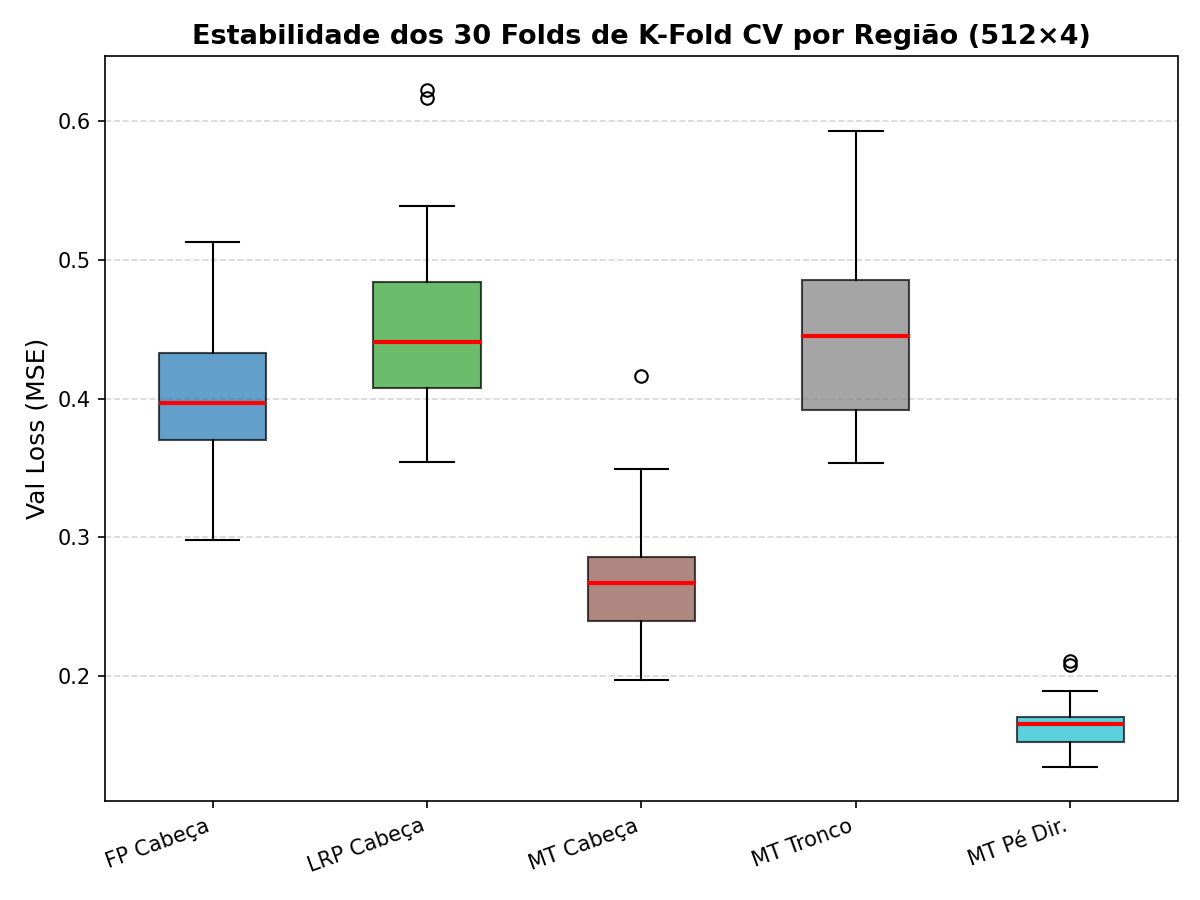
\includegraphics[width=\linewidth]{regioes/graficos/estabilidade_folds.png}
    \caption{Boxplot dos 30~folds por região.}
    \label{fig:estabilidade_box}
  \end{subfigure}
  \hfill
  \begin{subfigure}[b]{0.44\linewidth}
    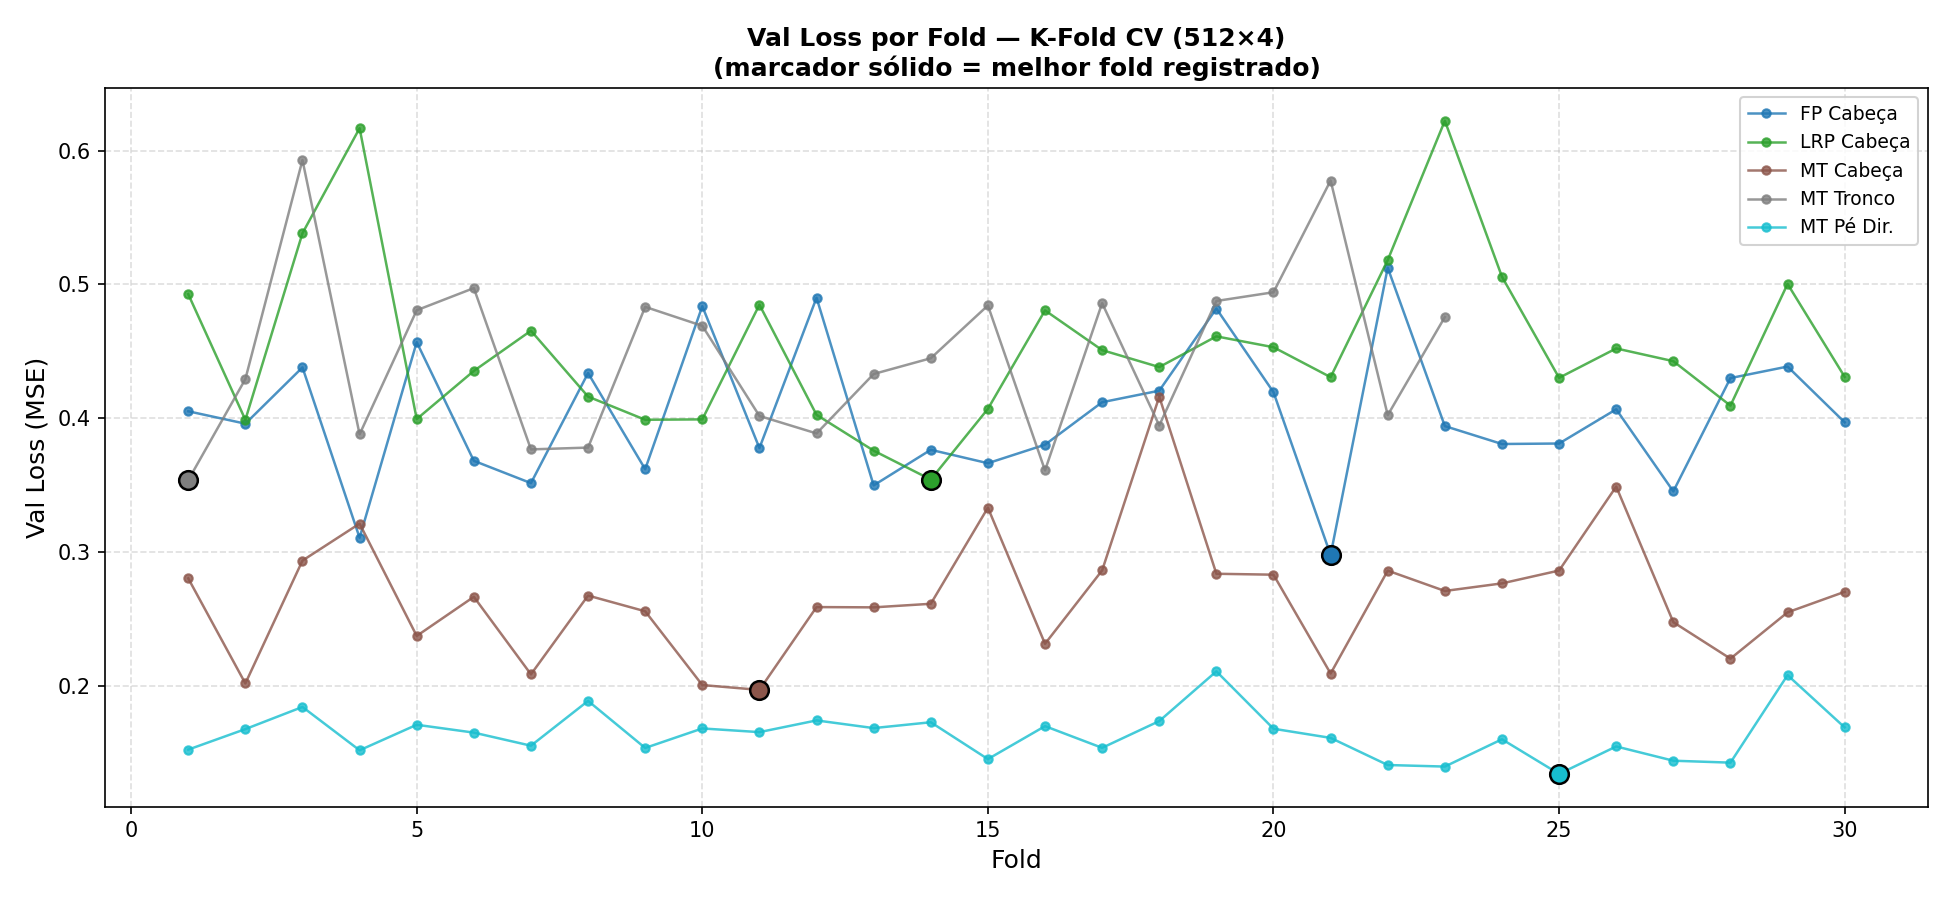
\includegraphics[width=\linewidth]{regioes/graficos/folds_scatter.png}
    \caption{Val.\ MSE por dobra (marcador = melhor fold).}
    \label{fig:estabilidade_scatter}
  \end{subfigure}
  \caption{%
    Distribuição e evolução do MSE de validação nos K-Fold por região
    (arquitetura $512 \times 4$).
  }
  \label{fig:estabilidade}
\end{figure}

\subsection{Análise por Variável --- Melhor Dobra}
\label{sec:por_variavel}

Para o modelo representativo de cada região (melhor dobra), calculam-se $R^2$
e MAE individuais por variável alvo. As
Figuras~\ref{fig:heatmap_r2} e~\ref{fig:heatmap_mae} apresentam esses
resultados em formato de mapa de calor.

\begin{figure}[htb]
  \centering
  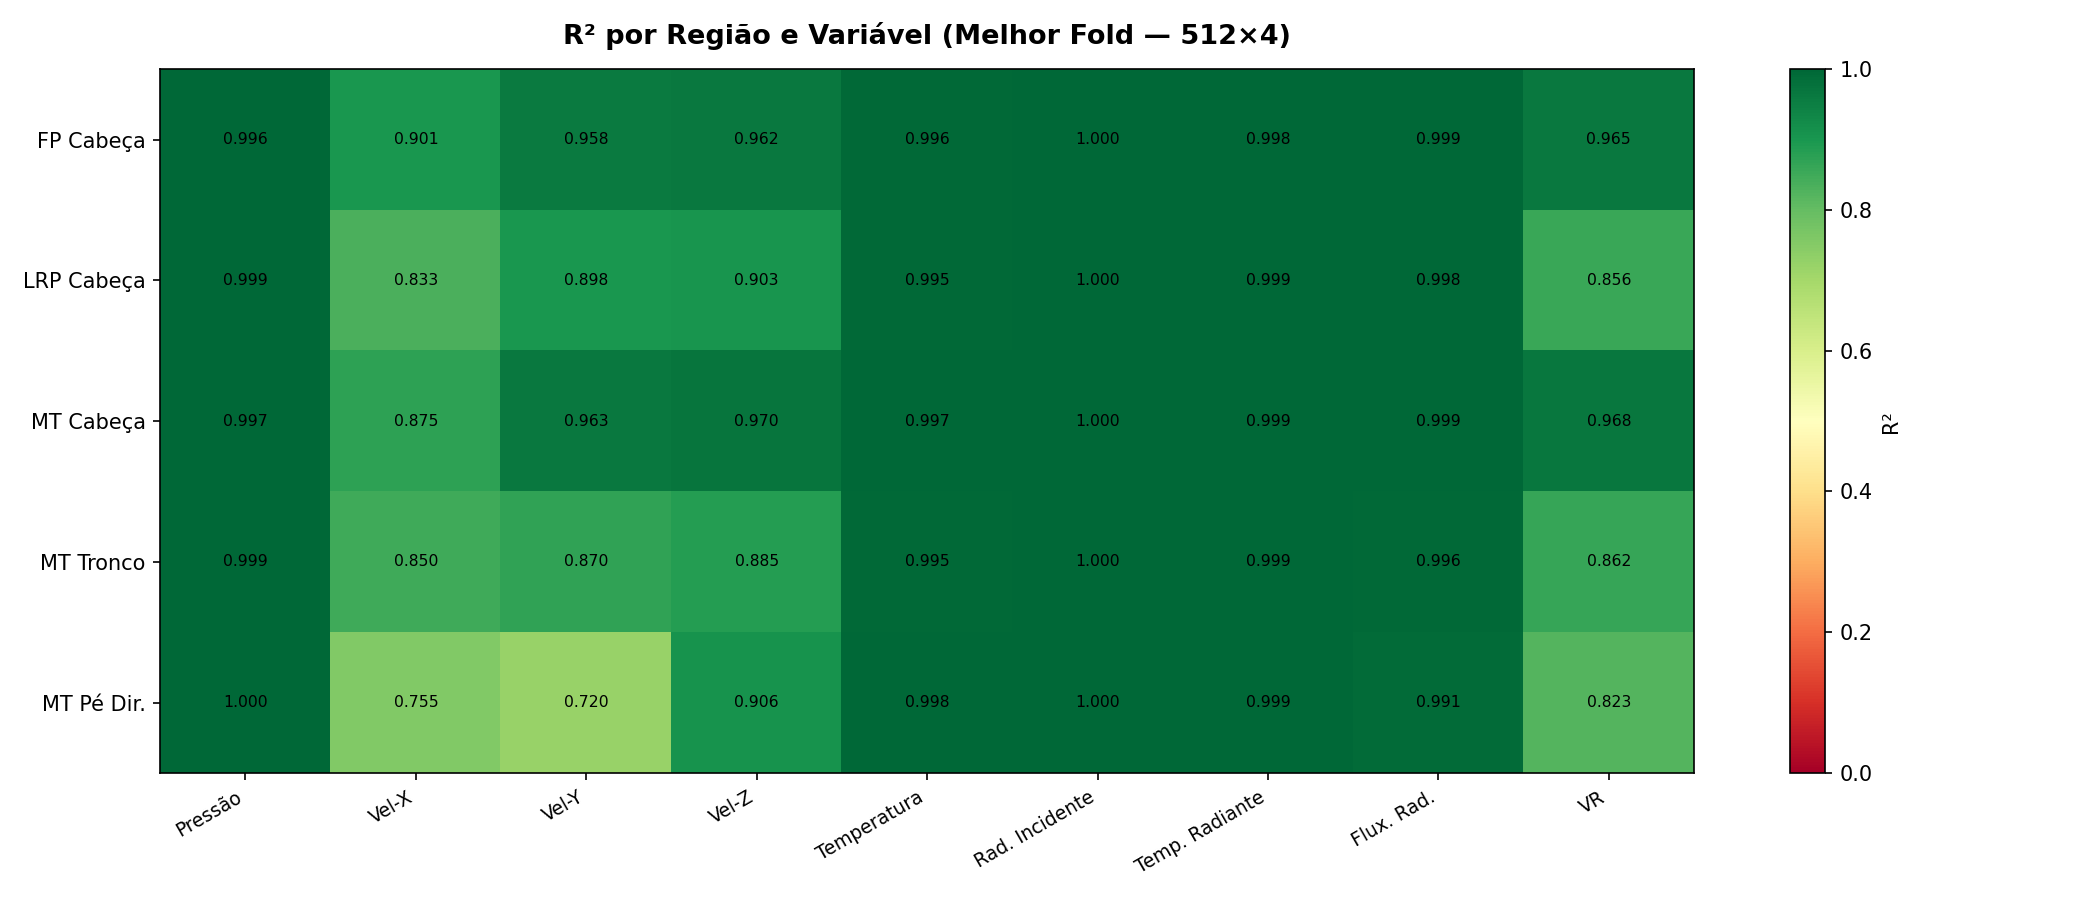
\includegraphics[width=\linewidth]{regioes/graficos/heatmap_r2.png}
  \caption{%
    Coeficiente de determinação $R^2$ da melhor dobra por região e variável
    de saída. Valores próximos de 1 (verde) indicam excelente predição;
    valores baixos (vermelho) indicam maior dificuldade do modelo.
    Regiões não treinadas serão adicionadas.
  }
  \label{fig:heatmap_r2}
\end{figure}

\begin{figure}[htb]
  \centering
  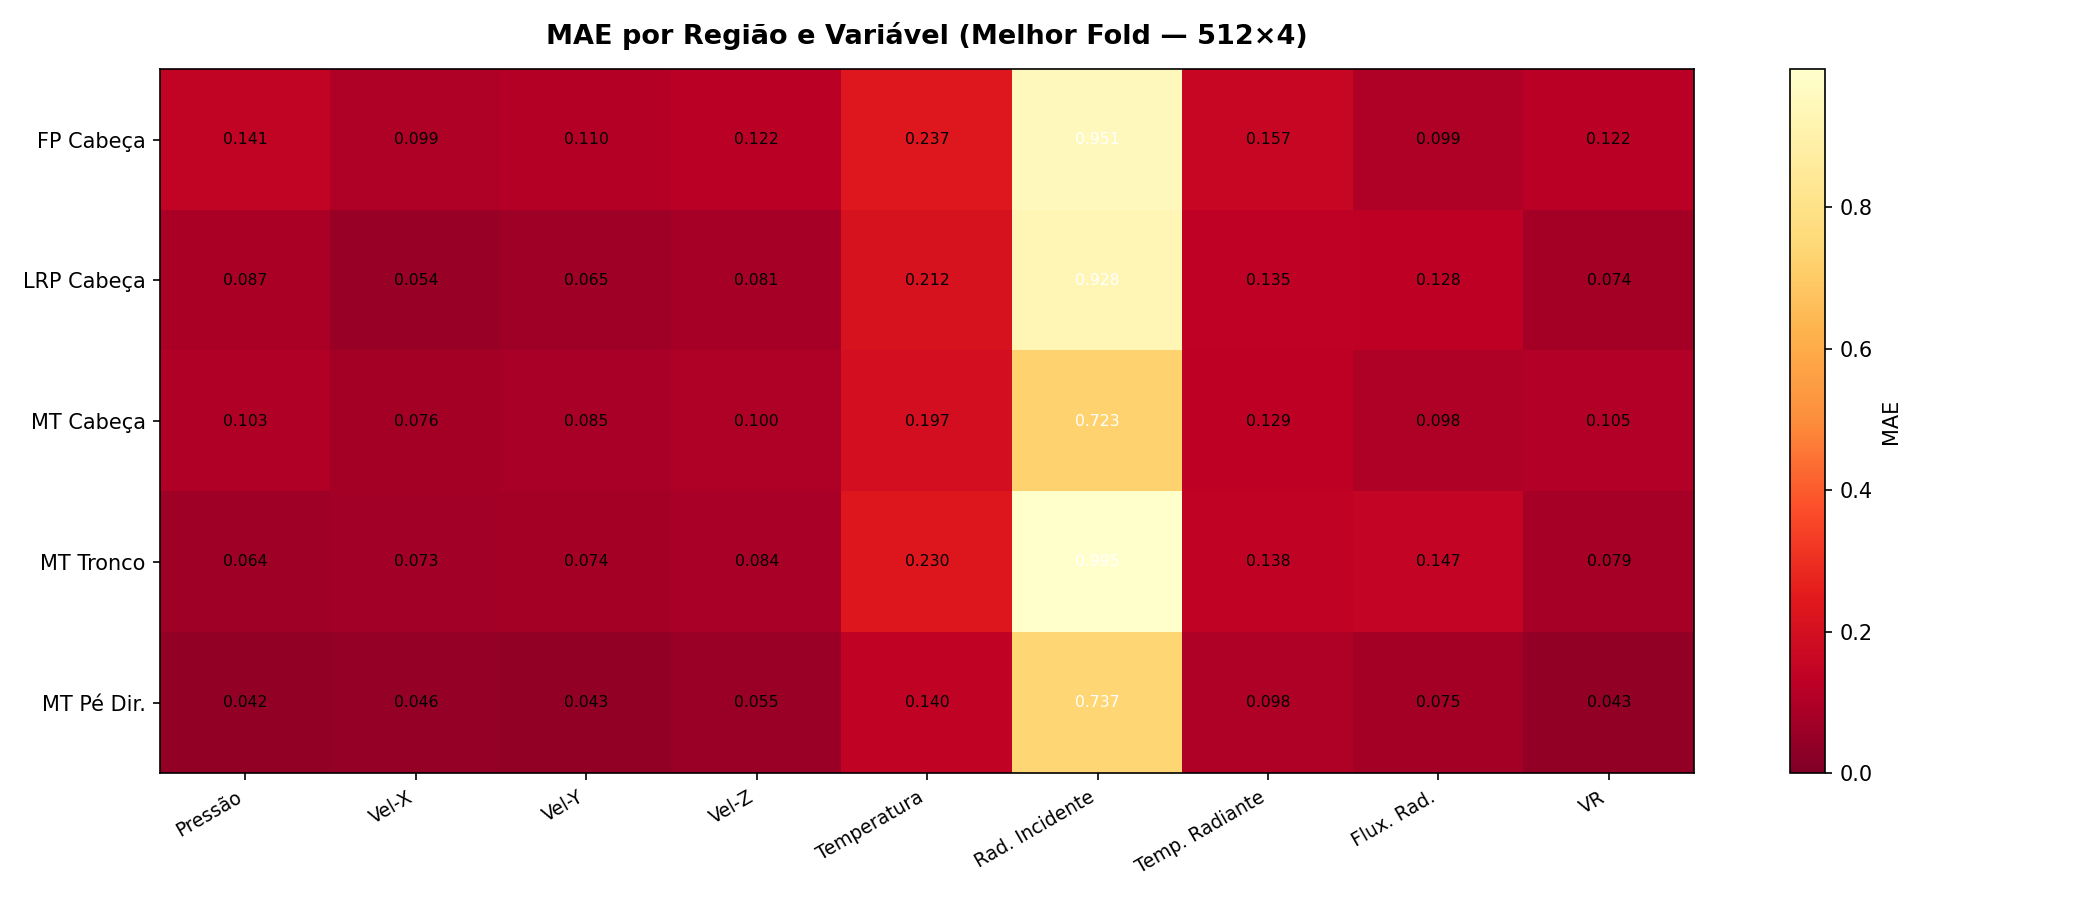
\includegraphics[width=\linewidth]{regioes/graficos/heatmap_mae.png}
  \caption{%
    Erro Absoluto Médio (MAE) da melhor dobra por região e variável de saída.
  }
  \label{fig:heatmap_mae}
\end{figure}

A Tabela~\ref{tab:r2_variaveis} sintetiza os valores de $R^2$ obtidos para
as quatro regiões treinadas.

\begin{table}[htb]
\centering
\caption{%
  Coeficiente de determinação $R^2$ da melhor dobra por região e variável
  ($512 \times 4$, sem L2). Regiões pendentes indicadas com ``--''.
}
\label{tab:r2_variaveis}
\setlength{\tabcolsep}{4pt}
\begin{tabular}{@{}lrrrrrrrrr@{}}
\toprule
\textbf{Região} &
  $p$ & $u$ & $v$ & $w$ & $T$ & $G$ & $T_r$ & $q_r$ & $v_r$ \\
\midrule
\textit{mt\_head}  & \num{0,997} & \num{0,875} & \num{0,963} & \num{0,970} & \num{0,997} & \num{1,000} & \num{0,999} & \num{0,999} & \num{0,968} \\
\textit{fp\_head}  & \num{0,996} & \num{0,901} & \num{0,958} & \num{0,962} & \num{0,996} & \num{1,000} & \num{0,998} & \num{0,999} & \num{0,965} \\
\textit{lrp\_head} & \num{0,999} & \num{0,833} & \num{0,899} & \num{0,903} & \num{0,995} & \num{1,000} & \num{0,999} & \num{0,998} & \num{0,856} \\
\textit{mt\_core}  & \num{0,999} & \num{0,850} & \num{0,870} & \num{0,885} & \num{0,995} & \num{1,000} & \num{0,999} & \num{0,996} & \num{0,862} \\
\midrule
\textit{rrp\_head}   & \andamento & \andamento & \andamento & \andamento & \andamento & \andamento & \andamento & \andamento & \andamento \\
\textit{mt\_l\_foot} & \andamento & \andamento & \andamento & \andamento & \andamento & \andamento & \andamento & \andamento & \andamento \\
\textit{mt\_r\_foot} & \num{1,000} & \num{0,755} & \num{0,720} & \num{0,907} & \num{0,998} & \num{1,000} & \num{0,999} & \num{0,991} & \num{0,823} \\
\midrule
\textit{rrp\_head}   & \andamento & \andamento & \andamento & \andamento & \andamento & \andamento & \andamento & \andamento & \andamento \\
\textit{mt\_l\_foot} & \andamento & \andamento & \andamento & \andamento & \andamento & \andamento & \andamento & \andamento & \andamento \\
\textit{outlet}      & \andamento & \andamento & \andamento & \andamento & \andamento & \andamento & \andamento & \andamento & \andamento \\
\bottomrule
\end{tabular}
{\small\\\textit{$p$: pressão; $u,v,w$: velocidades; $T$: temperatura;
  $G$: rad.\ incidente; $T_r$: temp.\ radiante; $q_r$: fluxo radiativo;
  $v_r$: vel.\ resultante.}}
\end{table}

Os resultados revelam um padrão consistente entre regiões: as variáveis de
pressão ($p$), temperatura ($T$), radiação incidente ($G$),
temperatura radiante ($T_r$) e fluxo radiativo ($q_r$) apresentam $R^2 > 0{,}99$
em todas as regiões avaliadas, demonstrando predição praticamente perfeita.
As componentes de velocidade ($u$, $v$, $w$, $v_r$) exibem $R^2$ entre
\num{0,83} e \num{0,97}, ainda satisfatórios considerando a natureza turbulenta
e tridimensional do escoamento.

\subsection{Distribuição Cumulativa dos Erros Absolutos}
\label{sec:cdf}

A distribuição cumulativa (CDF) dos erros absolutos ponto a ponto, agregada
sobre todos os 30~folds, permite avaliar o comportamento estatístico do erro
para toda a população de pontos CFD.
A Figura~\ref{fig:cdf_fp} apresenta este resultado para a região
\textit{fp\_head}.

\begin{figure}[htb]
  \centering
  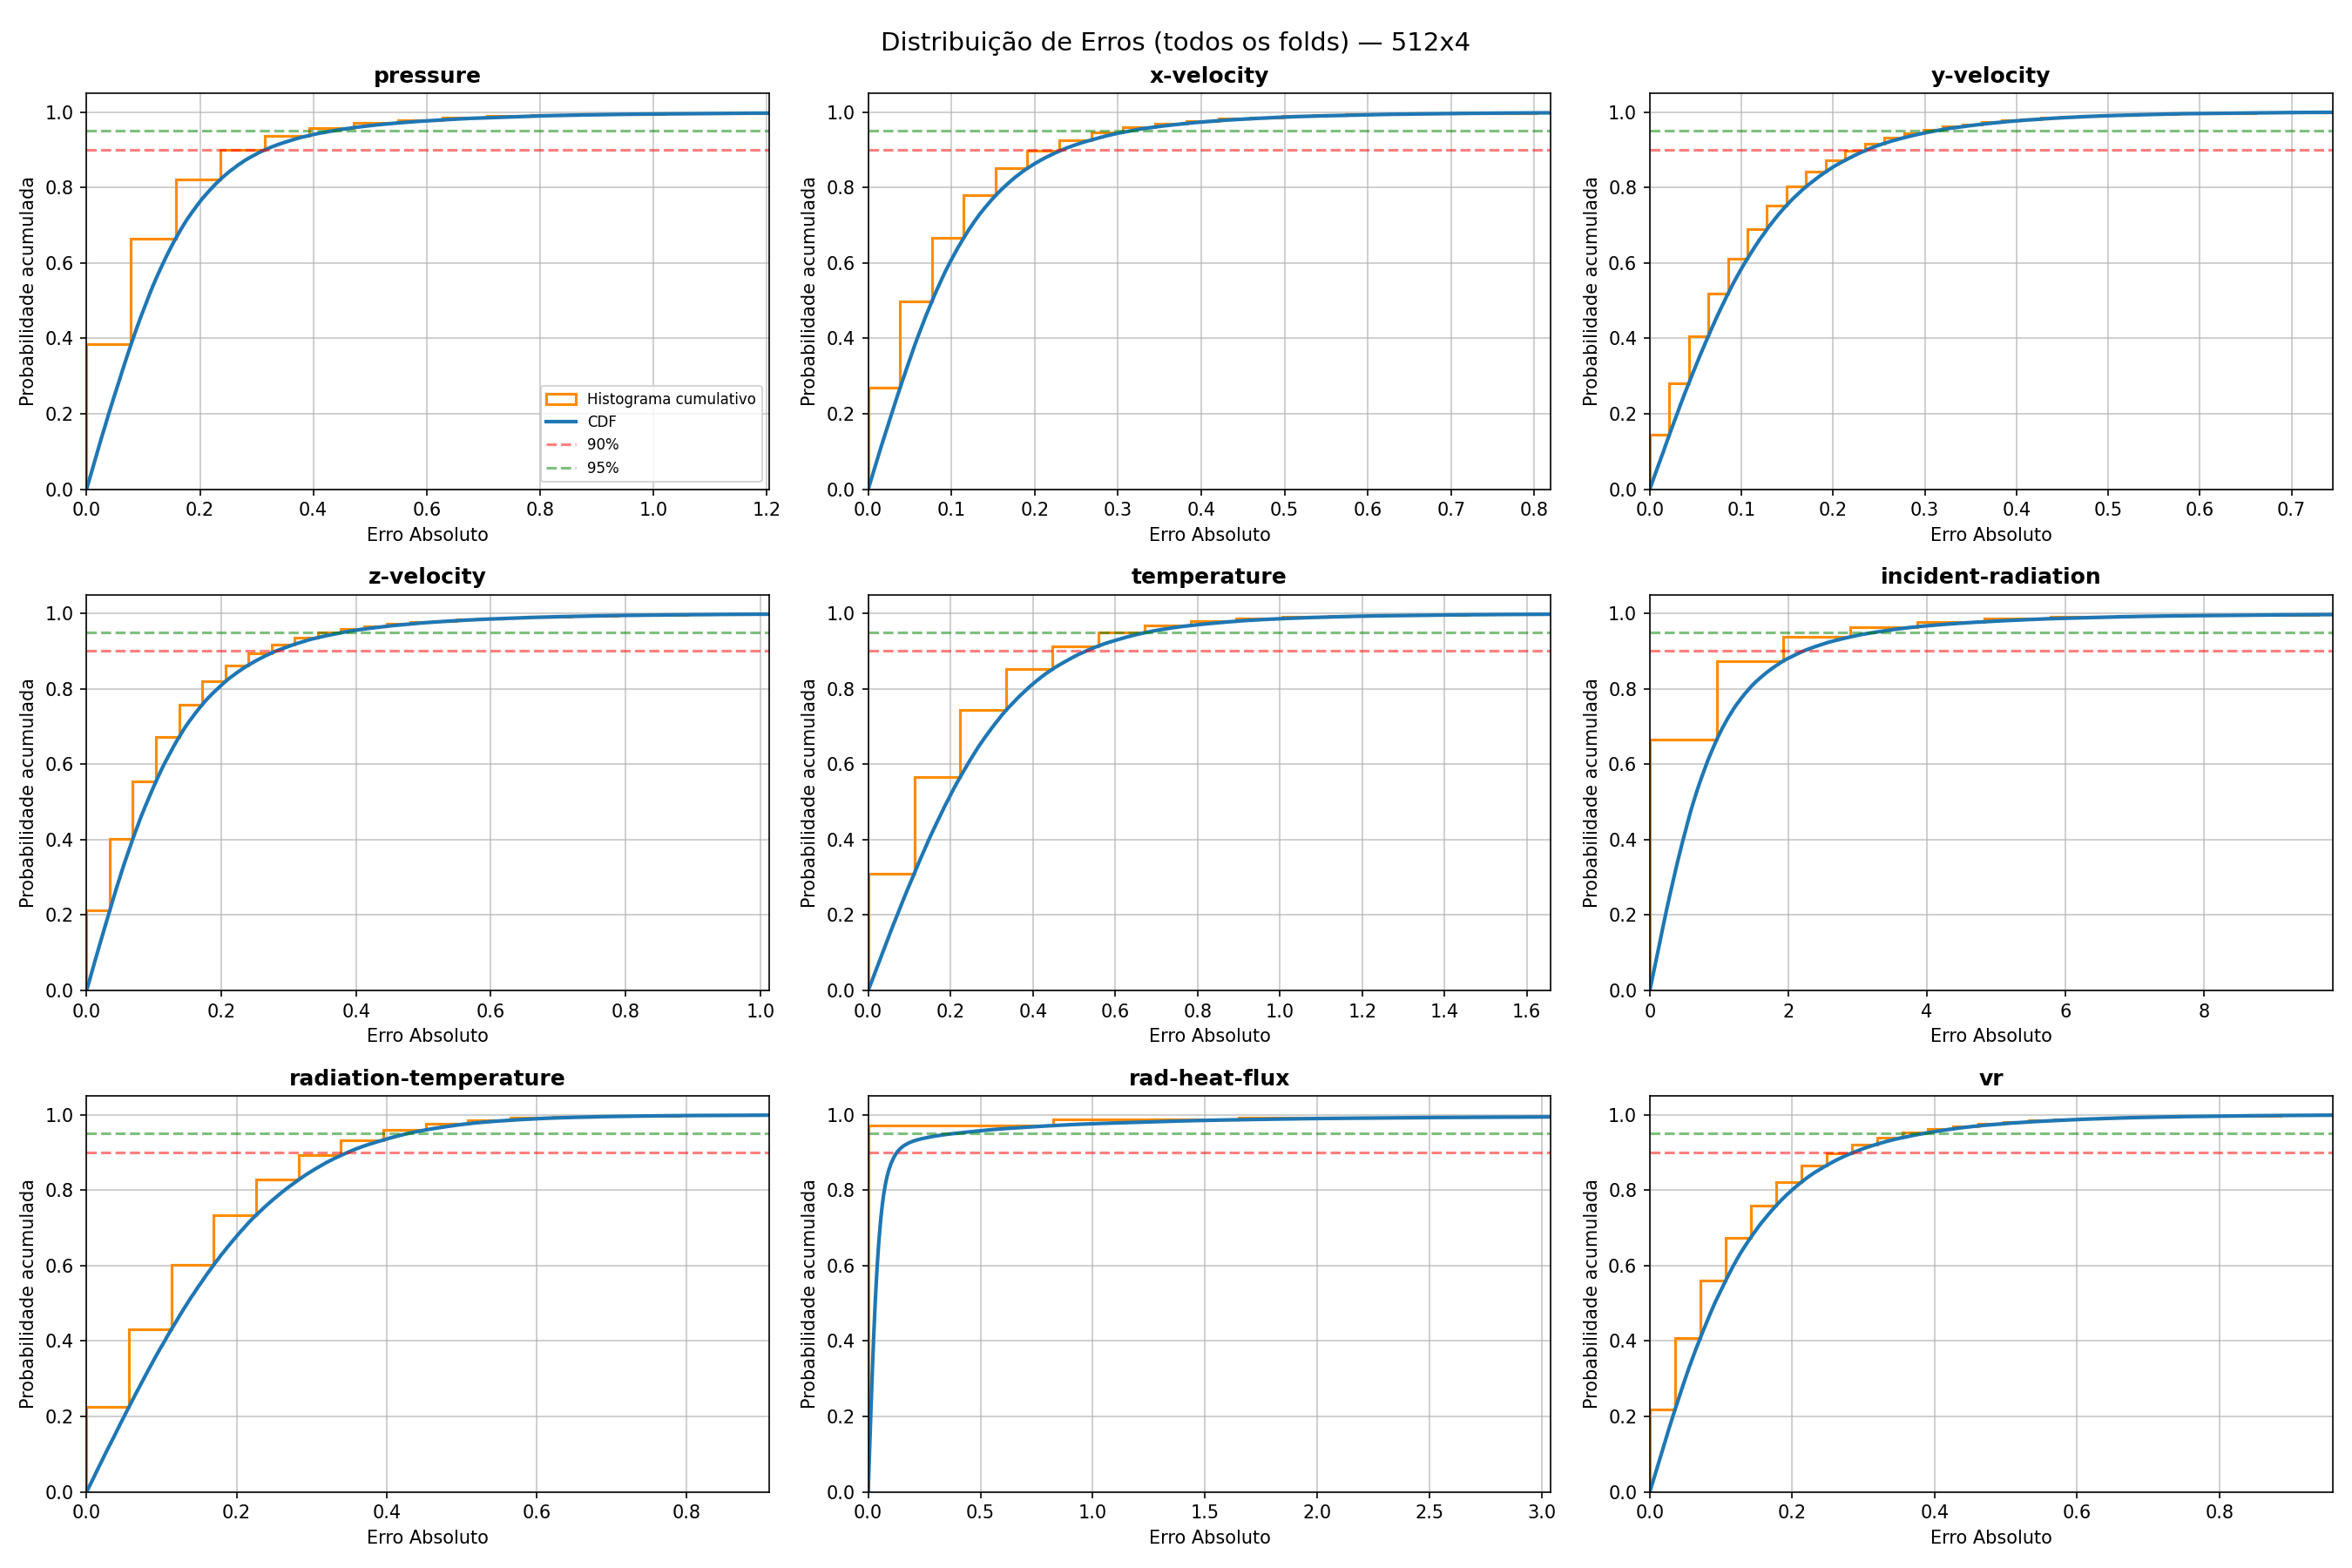
\includegraphics[width=\linewidth]{regioes/fp_head/graficos/hist_cumulativo/hist_cumulativo_512x4_fp_head.png}
  \caption{%
    Distribuição cumulativa dos erros absolutos por variável de saída,
    agregada sobre os 30~folds de K-Fold --- região \textit{fp\_head}.
    As linhas tracejadas indicam os percentis 90\% (vermelho) e 95\% (verde).
  }
  \label{fig:cdf_fp}
\end{figure}

\subsection{Comparação Visual: CFD Real versus Rede Neural}
\label{sec:comparacao_visual}

A qualidade das predições espaciais é avaliada por meio de mapas de calor
tridimensionais e gráficos de contorno em seções da cabine,
para a região \textit{fp\_head} (melhor dobra: fold~21,
$\text{MSE}_\text{val} = \num{0,2981}$).

\subsubsection{Campos de Pressão}

\begin{figure}[htb]
  \centering
  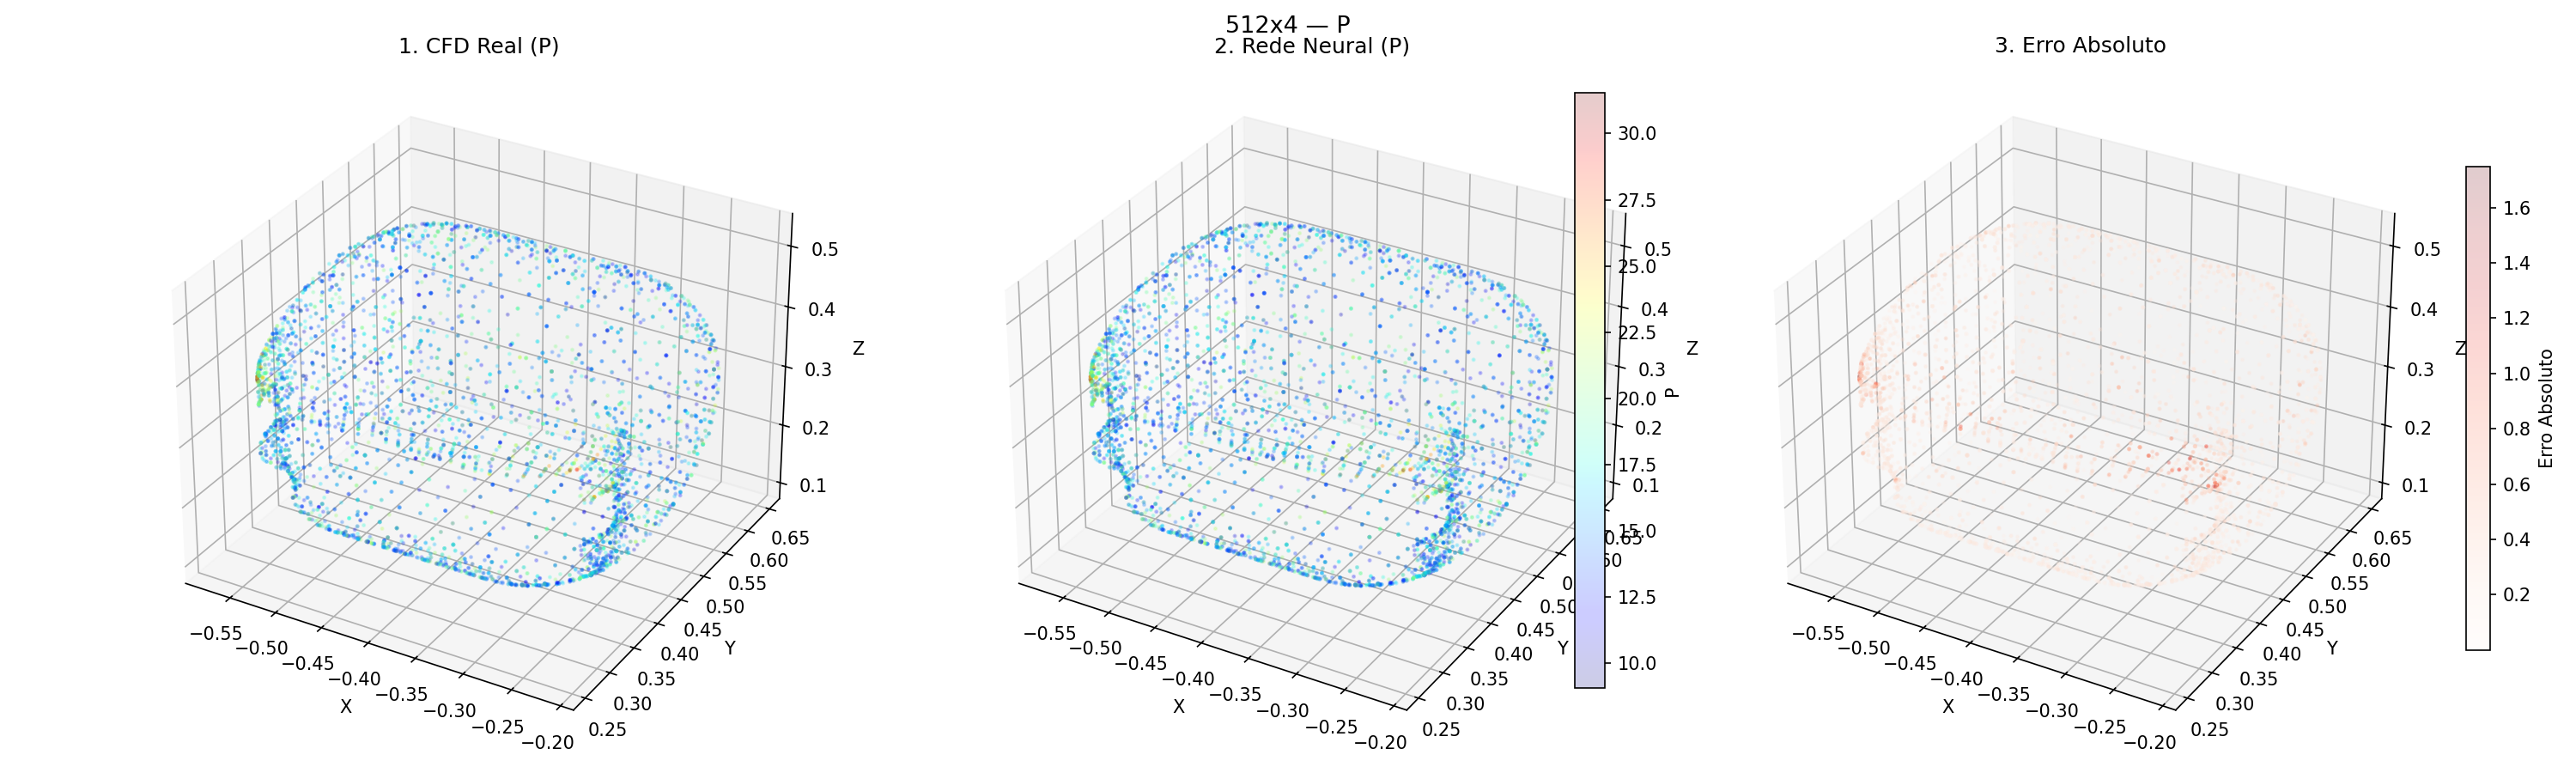
\includegraphics[width=\linewidth]{regioes/fp_head/graficos/heatmap/512x4_fp_head/heatmap_P_512x4_fp_head.png}
  \caption{%
    Campo de pressão ($p$): CFD de referência (esquerda), predição da rede
    neural (centro) e erro absoluto (direita) --- região \textit{fp\_head},
    fold~21 ($R^2 = \num{0,996}$).
  }
  \label{fig:heatmap_P}
\end{figure}

\begin{figure}[htb]
  \centering
  \begin{subfigure}[b]{0.48\linewidth}
    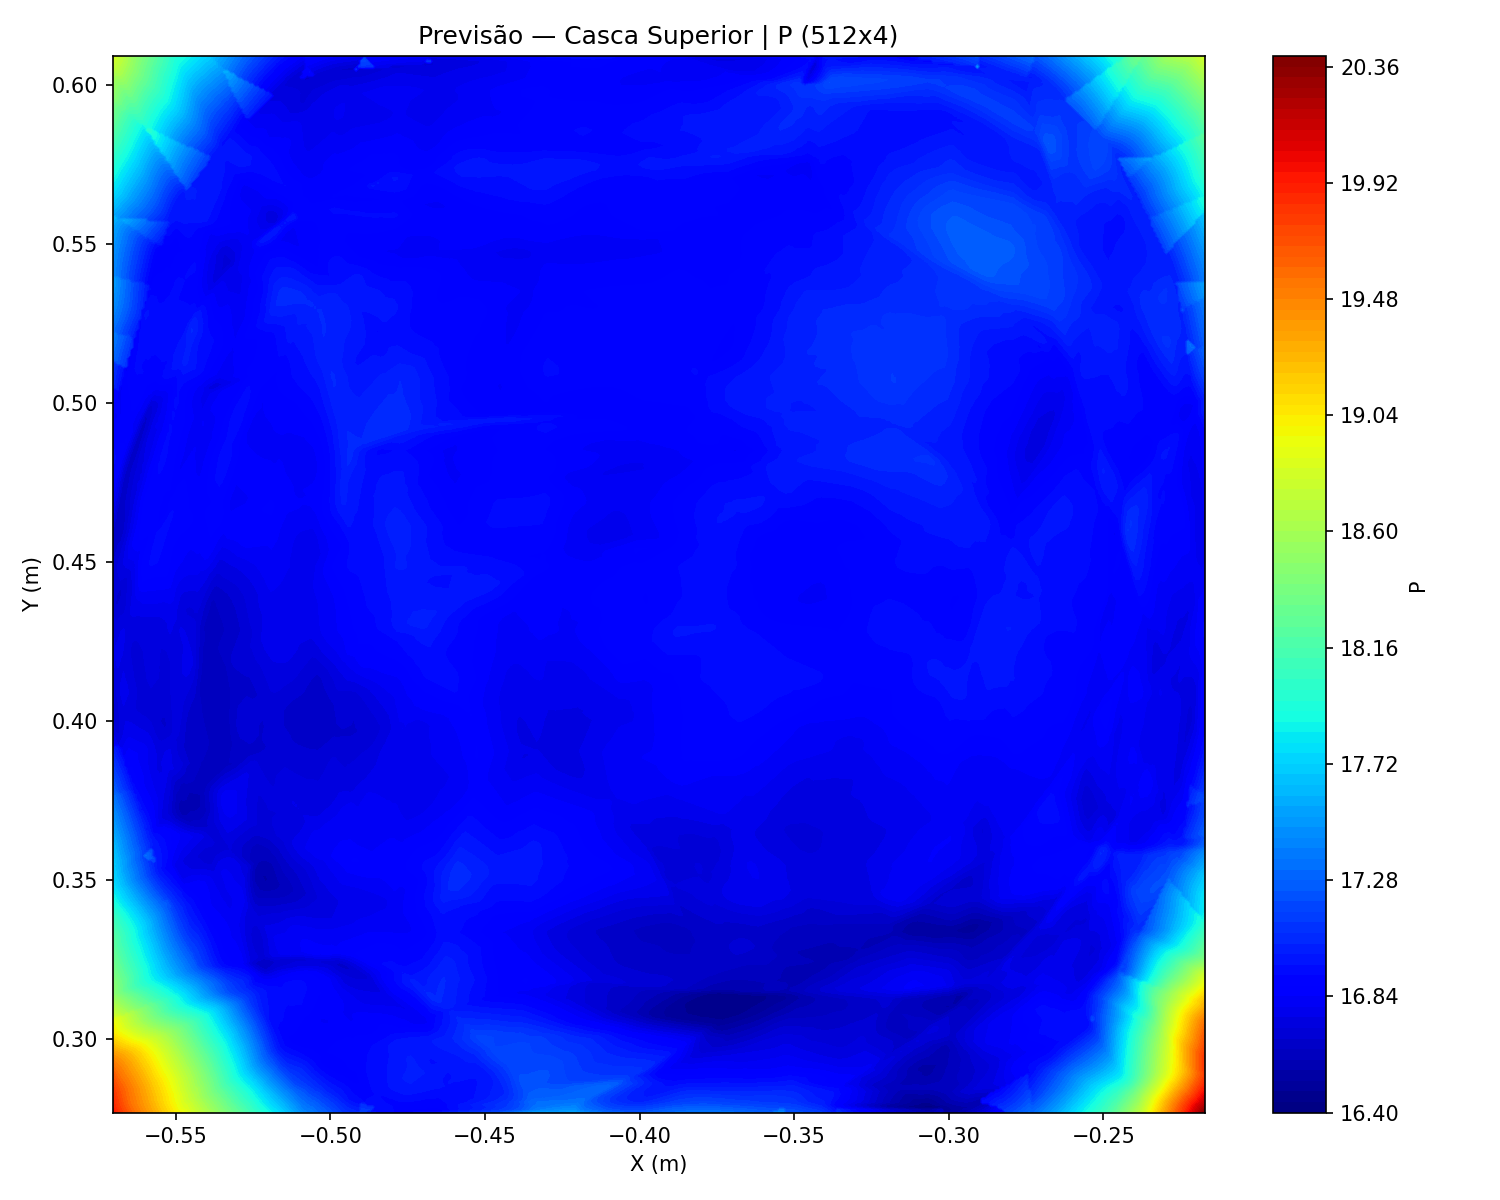
\includegraphics[width=\linewidth]{regioes/fp_head/graficos/contour/512x4_fp_head/contour_P_512x4_fp_head.png}
    \caption{Contorno de pressão.}
  \end{subfigure}
  \hfill
  \begin{subfigure}[b]{0.48\linewidth}
    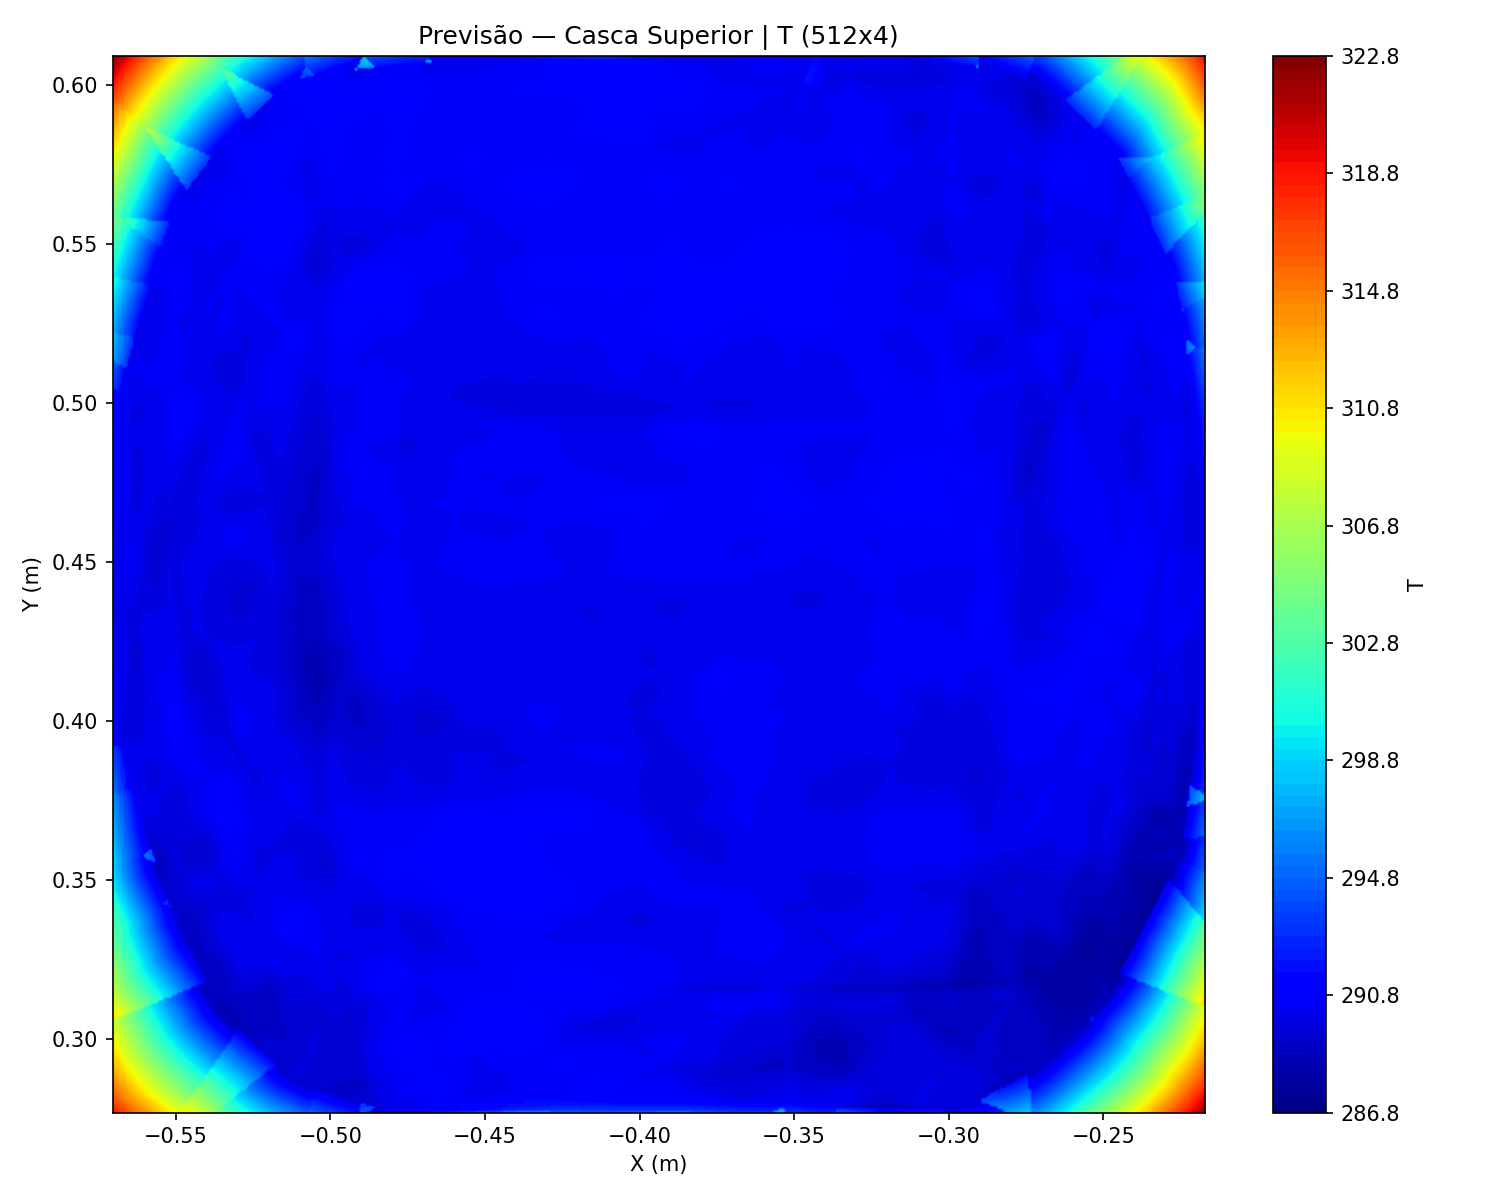
\includegraphics[width=\linewidth]{regioes/fp_head/graficos/contour/512x4_fp_head/contour_T_512x4_fp_head.png}
    \caption{Contorno de temperatura.}
  \end{subfigure}
  \caption{%
    Contornos 2D interpolados (via \textit{griddata}) na casca superior do
    domínio --- pressão ($p$) e temperatura ($T$), região \textit{fp\_head}.
  }
  \label{fig:contour}
\end{figure}

\subsubsection{Campo de Temperatura}

\begin{figure}[htb]
  \centering
  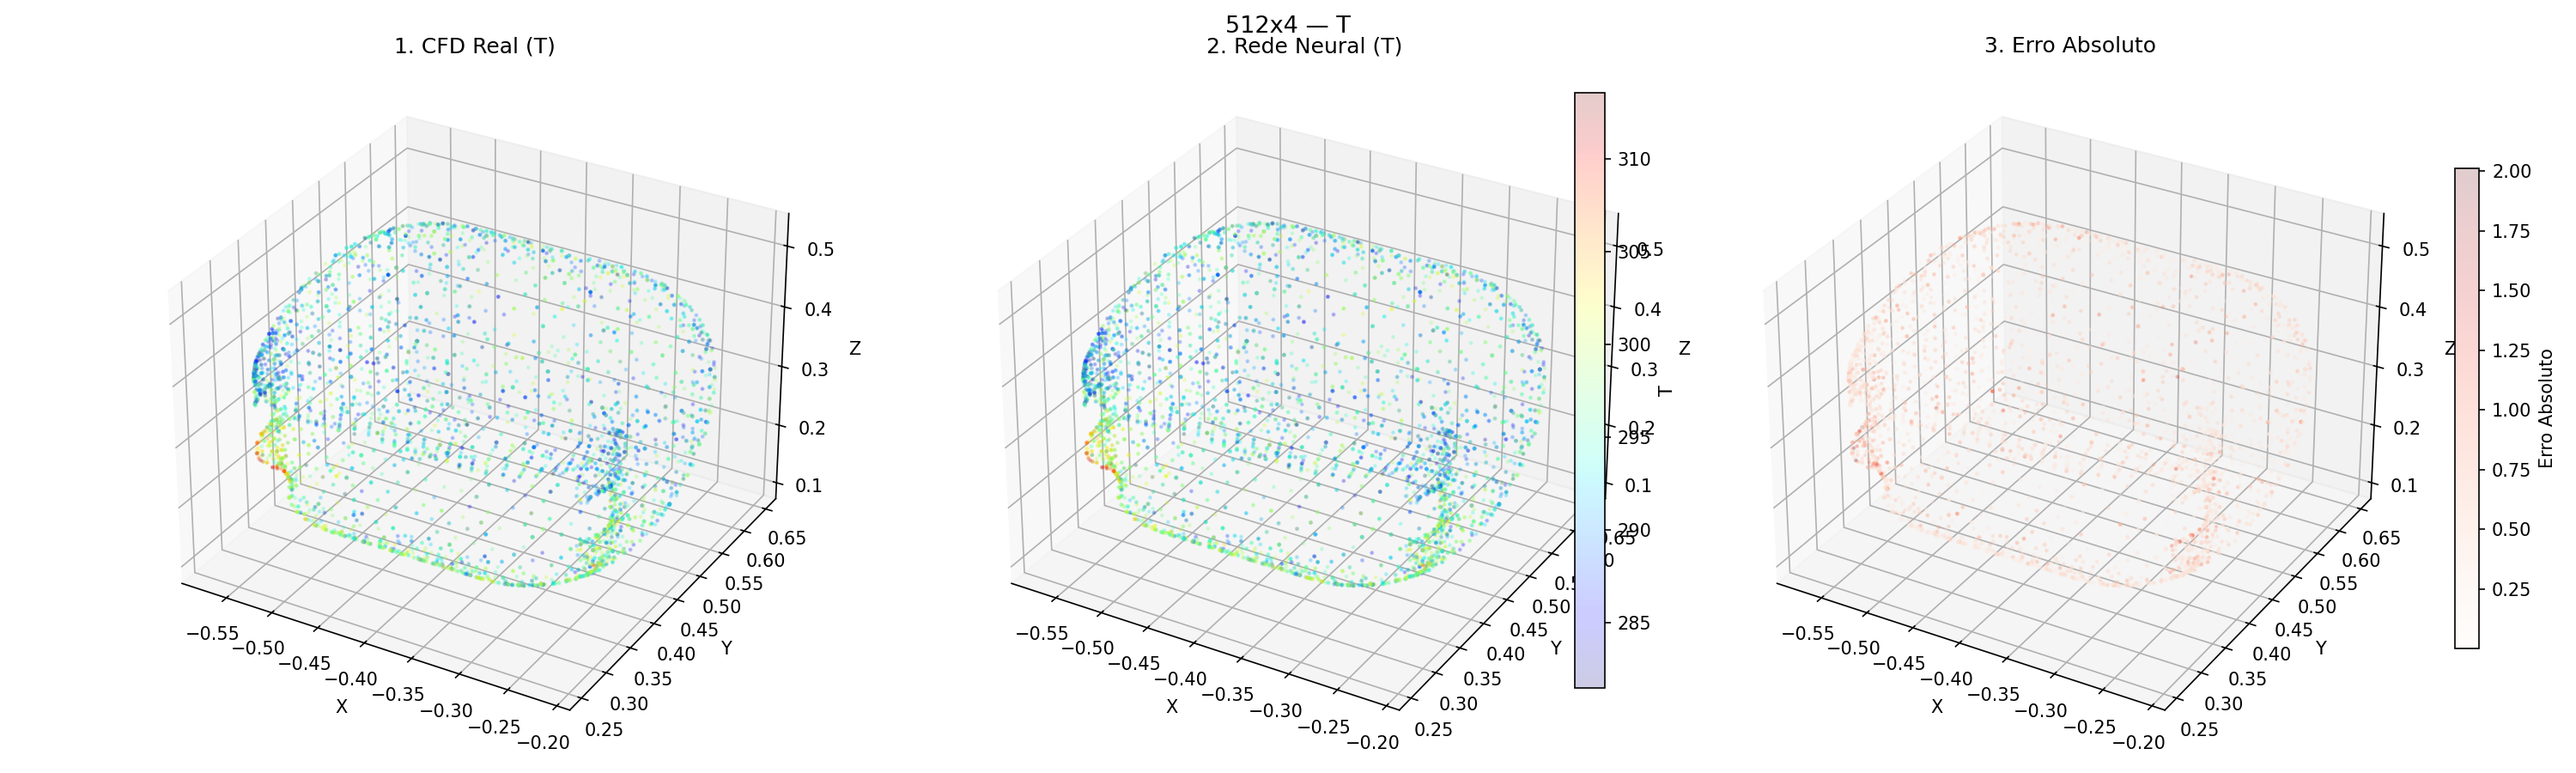
\includegraphics[width=\linewidth]{regioes/fp_head/graficos/heatmap/512x4_fp_head/heatmap_T_512x4_fp_head.png}
  \caption{%
    Campo de temperatura ($T$): CFD de referência (esquerda), predição da rede
    neural (centro) e erro absoluto (direita) --- região \textit{fp\_head},
    fold~21 ($R^2 = \num{0,996}$).
  }
  \label{fig:heatmap_T}
\end{figure}

\subsubsection{Região \textit{mt\_r\_foot} --- Pé Direito do Motorista}

\begin{figure}[htb]
  \centering
  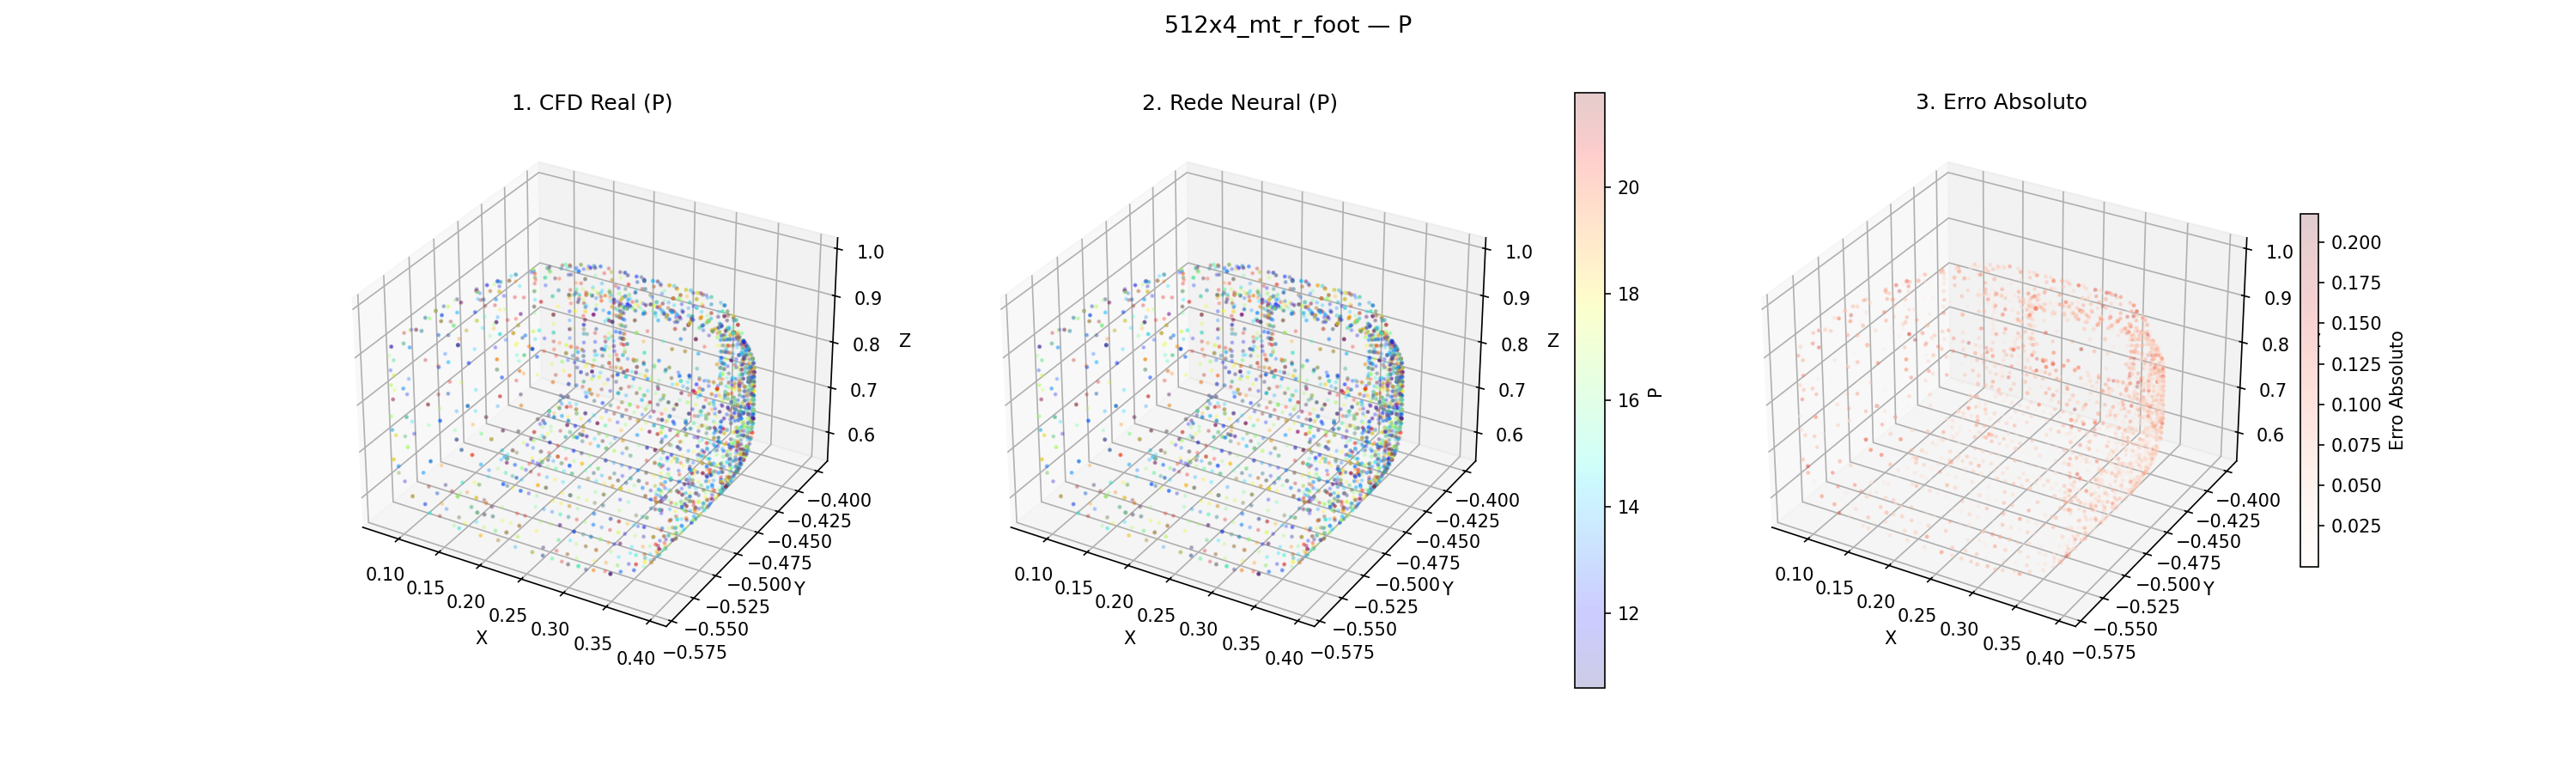
\includegraphics[width=\linewidth]{regioes/mt_r_foot/graficos/heatmap/512x4_mt_r_foot/heatmap_P_512x4_mt_r_foot.png}
  \caption{%
    Campo de pressão ($p$): CFD de referência, predição da rede neural e erro
    absoluto --- região \textit{mt\_r\_foot}, fold~25
    ($R^2 = \num{1,000}$).
  }
  \label{fig:heatmap_P_foot}
\end{figure}

\begin{figure}[htb]
  \centering
  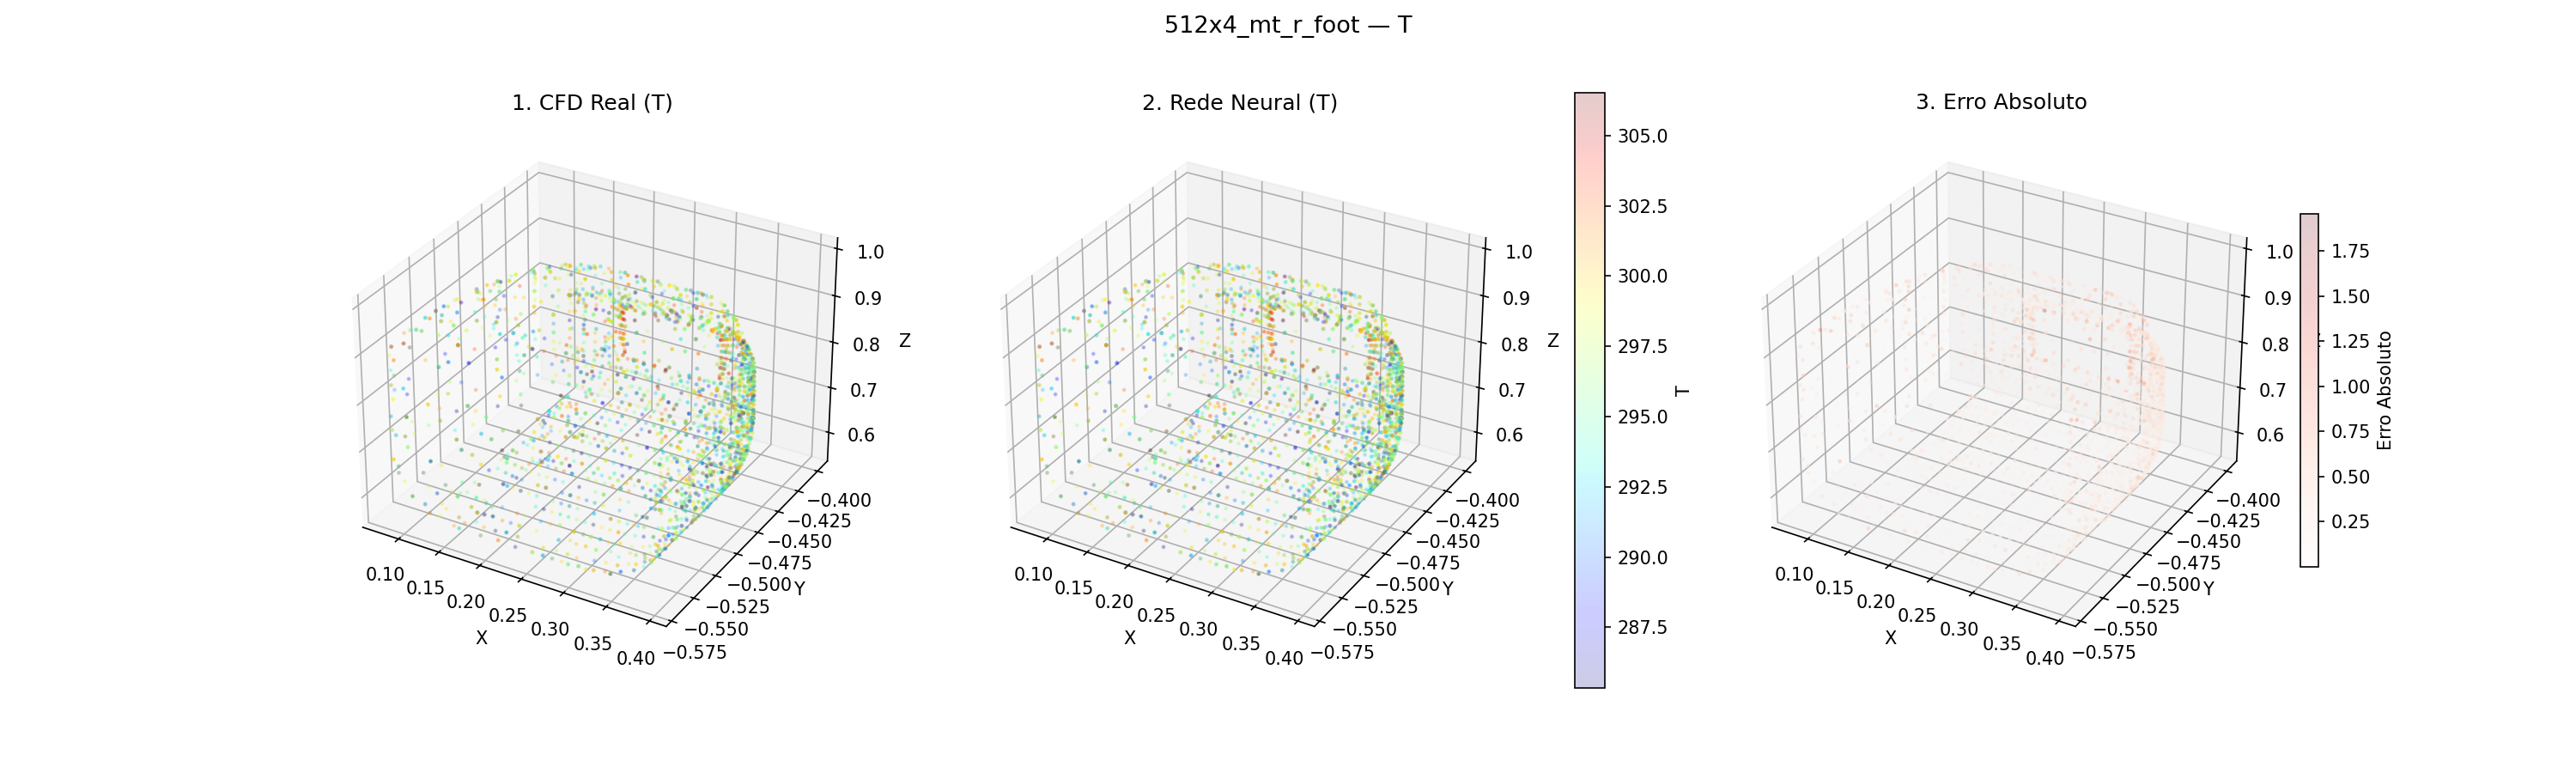
\includegraphics[width=\linewidth]{regioes/mt_r_foot/graficos/heatmap/512x4_mt_r_foot/heatmap_T_512x4_mt_r_foot.png}
  \caption{%
    Campo de temperatura ($T$): CFD de referência, predição da rede neural e
    erro absoluto --- região \textit{mt\_r\_foot}, fold~25
    ($R^2 = \num{0,998}$).
  }
  \label{fig:heatmap_T_foot}
\end{figure}

\begin{figure}[htb]
  \centering
  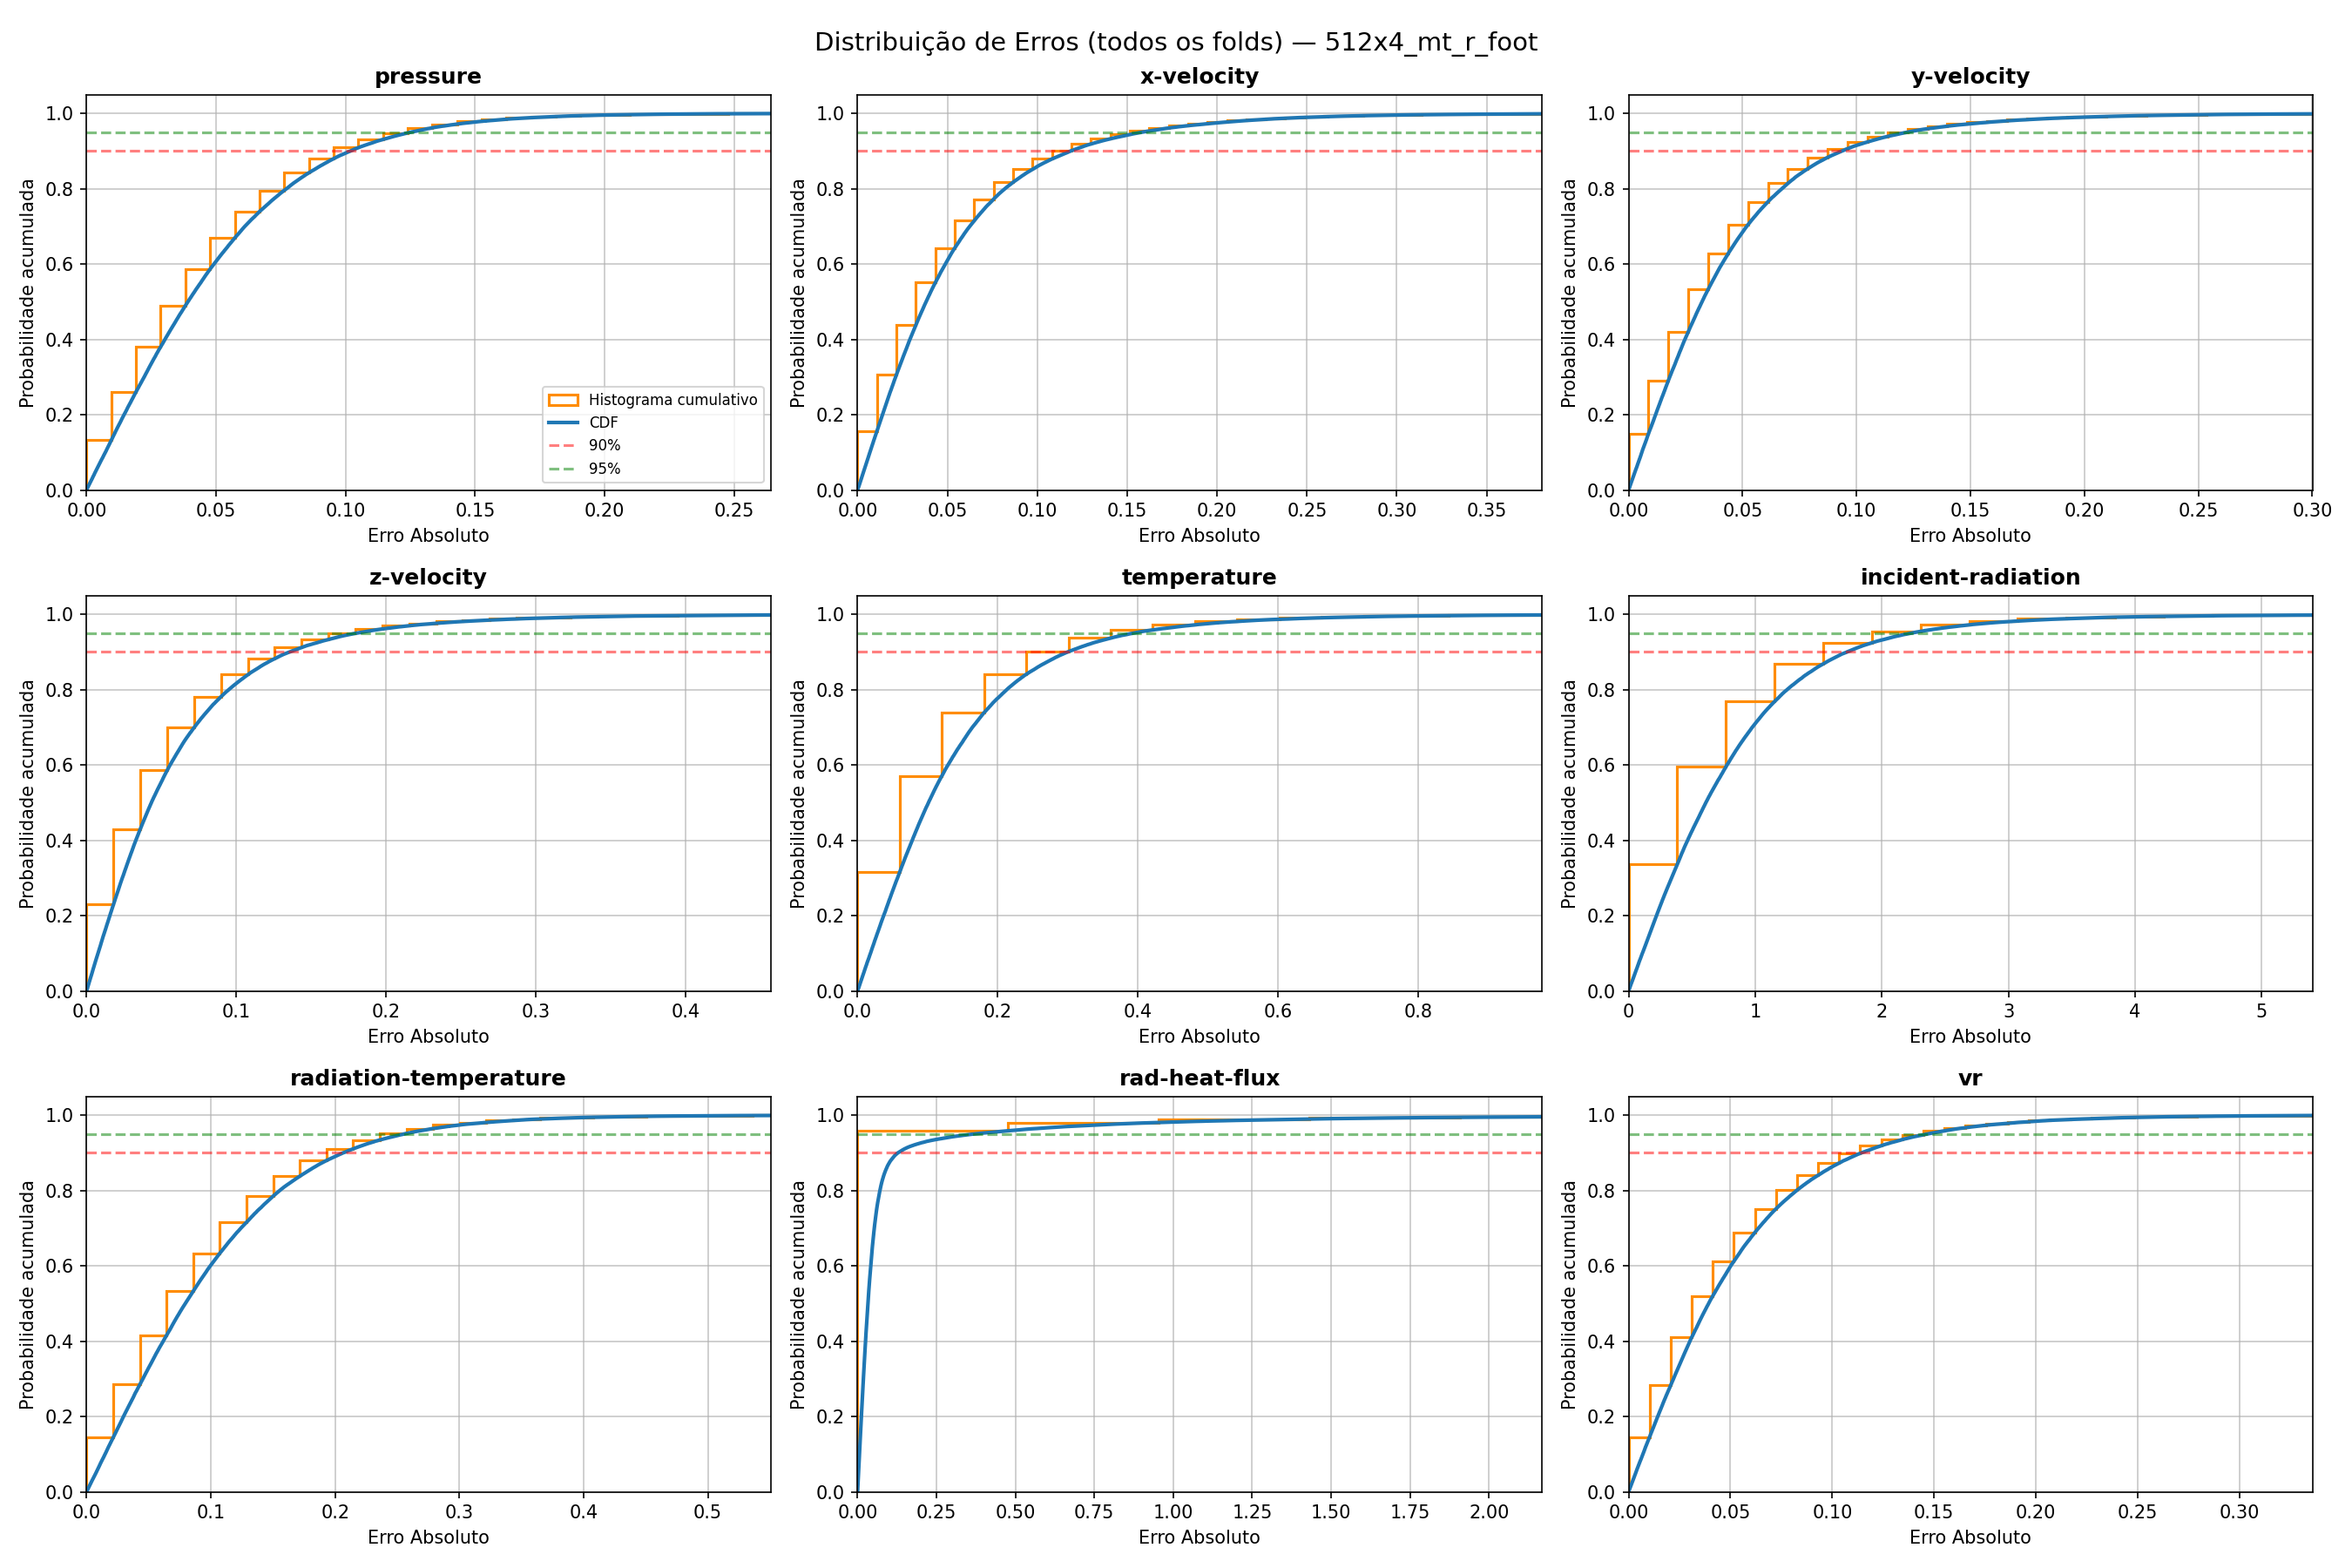
\includegraphics[width=\linewidth]{regioes/mt_r_foot/graficos/hist_cumulativo/hist_cumulativo_512x4_mt_r_foot.png}
  \caption{%
    Distribuição cumulativa dos erros absolutos por variável --- região
    \textit{mt\_r\_foot}, todos os 30~folds.
  }
  \label{fig:cdf_foot}
\end{figure}

\todo[inline]{%
  Inserir figuras para as regiões pendentes após conclusão dos treinamentos:
  \textit{rrp\_head}, \textit{mt\_l\_foot}, \textit{outlet}.
}

% =========================================================================
\section*{Referências}
\begin{thebibliography}{9}

\bibitem{mao2018}
MAO, Y.; JI WANG; JUNMING LI.
Experimental and numerical study of flow and heat transfer characteristics
in a passenger compartment.
\textit{International Journal of Thermal Sciences}, 2018.

\bibitem{medeiros2025}
MEDEIROS, M.~B.
\textit{Análise de parâmetros de conforto térmico de cabine por meio de
simulações CFD e redes neurais profundas}.
Dissertação (Mestrado em Engenharia e Ciências Mecânicas) ---
Universidade Federal de Santa Catarina, Joinville, 2025.

\bibitem{ashrae55}
ASHRAE.
\textit{ANSI/ASHRAE Standard 55: Thermal Environmental Conditions for
Human Occupancy}. Atlanta: ASHRAE, 2023.

\end{thebibliography}

\end{document}
